\section{Wasserphantom Teil 3}

\subsection{Bestrahlung verschiedener Volumina}

In diesem Aufgabenteil wird erneut ein Wasserphantom mit den Maßen
$20$x$20$x$20$ $\si{\centi\meter\tothe{3}}$, dem Schichtabstand
$\SI{0.25}{\centi\meter}$ und einem CT-Wert von Wasser.
Diesmal werden in dem Wasserphantom weitere Konturen definiert.
Es werden vier Kugeln mit einem Durchmesser von $\SI{2.5}{\centi\meter}$
und CT-Werten von Luft, Fett, Wasser und Knochen in das Wasserphantom
eingezeichnet. Dieses Wasserphantom wird nun mit mit einem
$25$x$25$ $\si{\centi\meter\squared}$ $\SI{6}{\mega\volt}$ Photonenfeld
bestrahlt bei einer Grantry Rotation von $90°$. Bei der Bestrahlung wird
die Bestrahlungsmaschine Eclipse-CAP-TB und der Berechnungsalgorithmus
Acuros verwendet. Diese Bestrahlung, ohne Normierung auf einen
Referenzpunkt, ist in Abbildung \ref{abb:3.1unnormiert} gezeigt.

\begin{figure}[H]
  \centering
  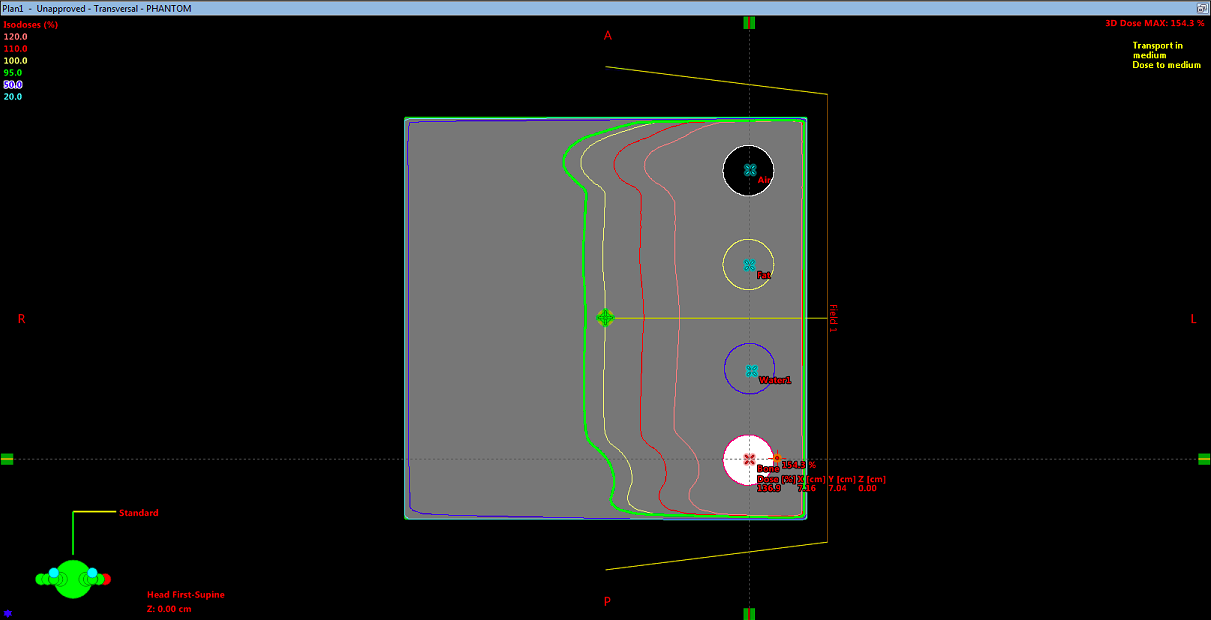
\includegraphics[width=\textwidth]{../../Wasserphantom Bilder/Aufgabe3.1_OhneReferenz.png}
  \caption{Isodosenlinien der Bestrahlung des modifizieren Wasserphantoms, ohne Normierung auf einen Referenzpunkt.}
  \label{abb:3.1unnormiert}
\end{figure}

Nun wird in den vier Strukturen jeweils ein Referenzpunkt festgelegt und der
Plan wird der Reihe nach auf die vier Referenzpunkte normiert. Die
Dosisverteilungen sind in den Abbildungen \ref{abb:3.1Luft},
\ref{abb:3.1Fett}, \ref{abb:3.1Wasser} und \ref{abb:3.1Knochen} dargestellt.

\begin{figure}[H]
  \centering
  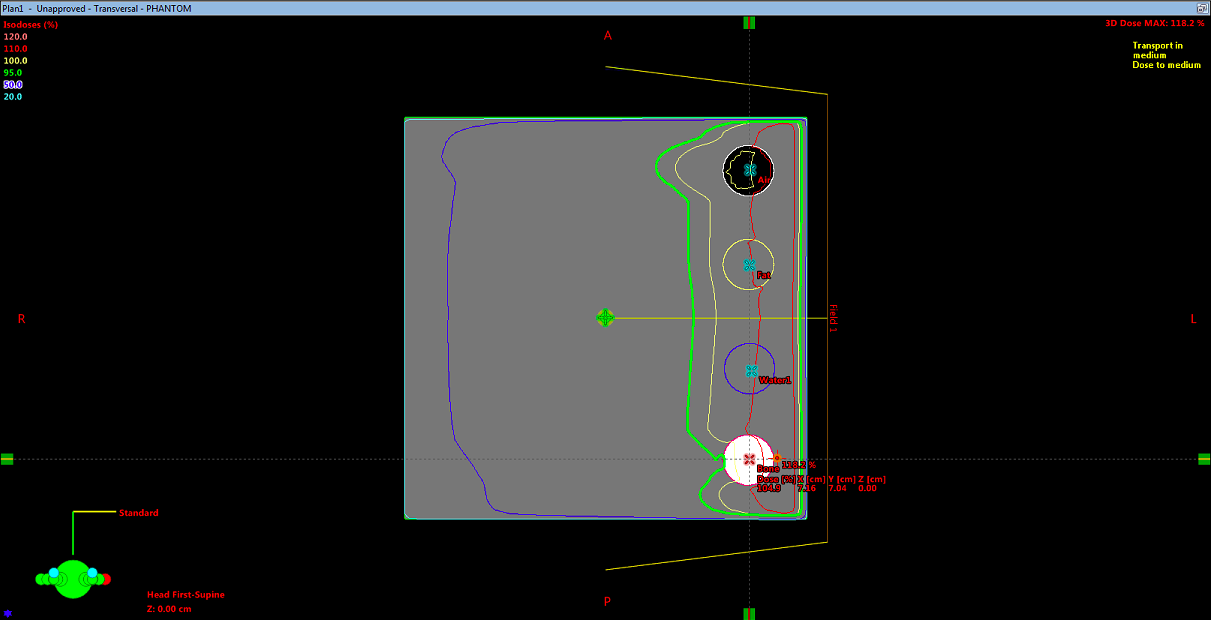
\includegraphics[width=\textwidth]{../../Wasserphantom Bilder/Aufgabe3.1_ReferenzLuft.png}
  \caption{Resultierende Dosisverteilungen im Wasserphantom bei Normierung auf den Referenzpunkt \enquote{Luft}.}
  \label{abb:3.1Luft}
\end{figure}

\begin{figure}[H]
  \centering
  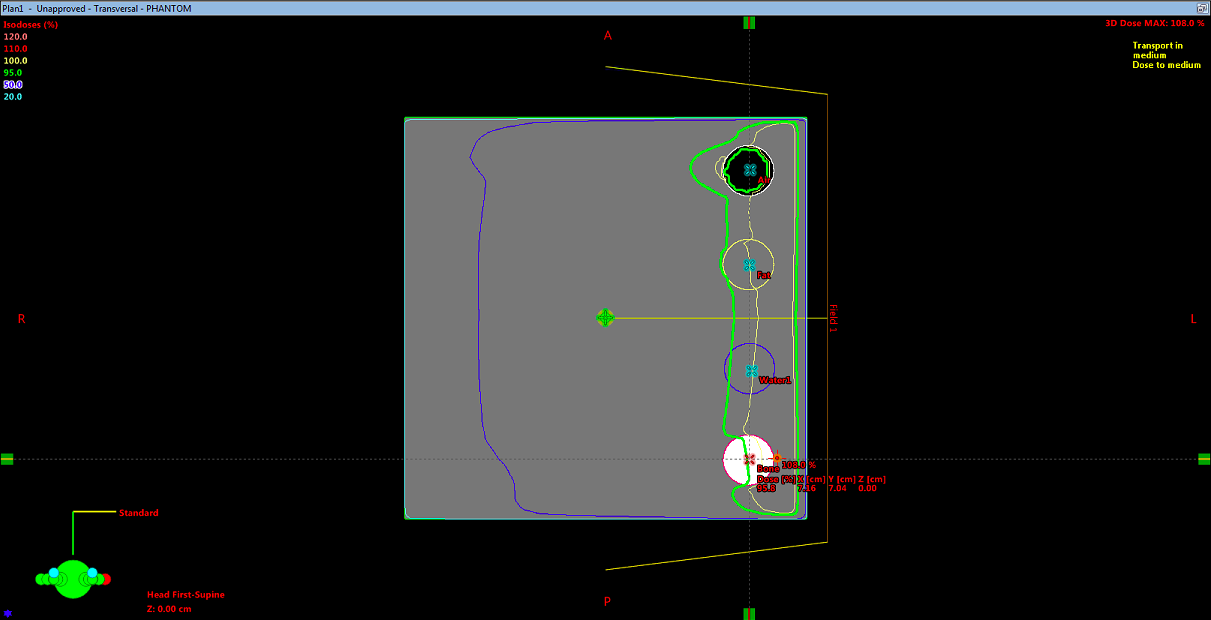
\includegraphics[width=\textwidth]{../../Wasserphantom Bilder/Aufgabe3.1_ReferenzFett.png}
  \caption{Resultierende Dosisverteilungen im Wasserphantom bei Normierung auf den Referenzpunkt \enquote{Fett}.}
  \label{abb:3.1Fett}
\end{figure}

\begin{figure}[H]
  \centering
  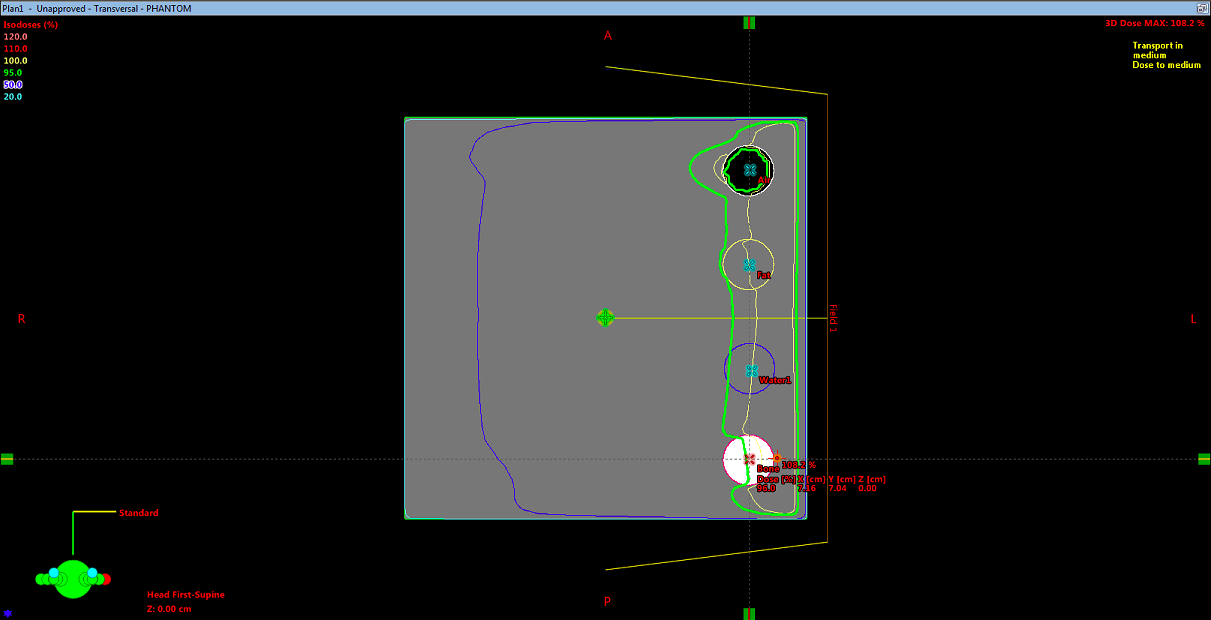
\includegraphics[width=\textwidth]{../../Wasserphantom Bilder/Aufgabe3.1_ReferenzWasser.png}
  \caption{Resultierende Dosisverteilungen im Wasserphantom bei Normierung auf den Referenzpunkt \enquote{Wasser}.}
  \label{abb:3.1Wasser}
\end{figure}

\begin{figure}[H]
  \centering
  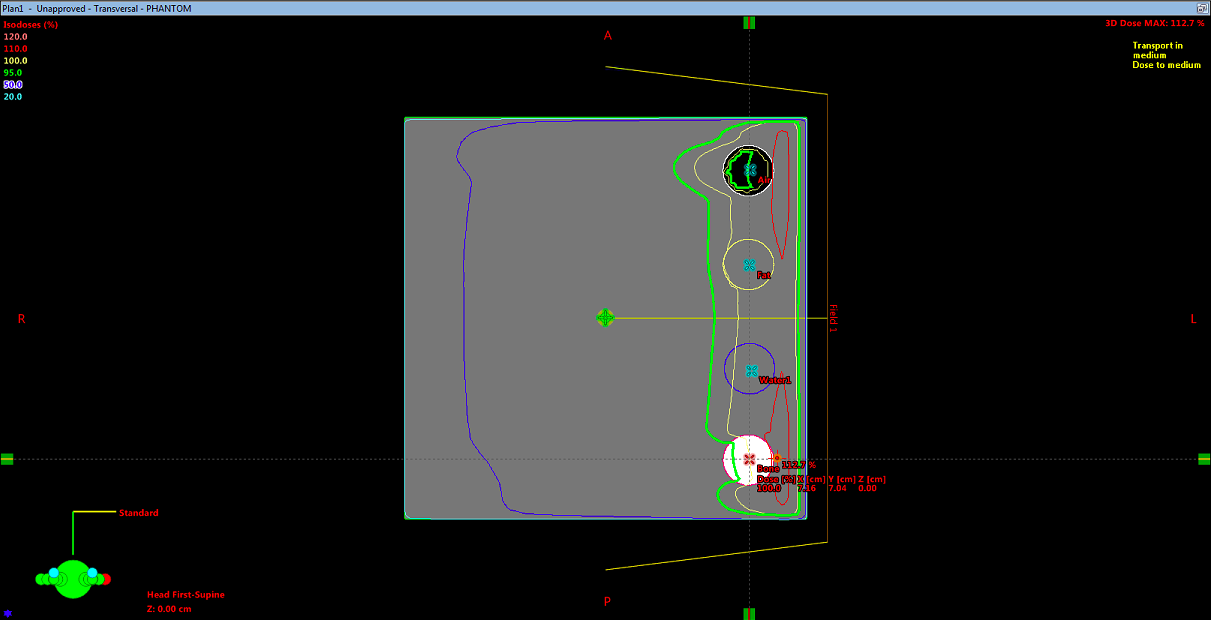
\includegraphics[width=\textwidth]{../../Wasserphantom Bilder/Aufgabe3.1_ReferenzKnochen.png}
  \caption{Resultierende Dosisverteilungen im Wasserphantom bei Normierung auf den Referenzpunkt \enquote{Knochen}.}
  \label{abb:3.1Knochen}
\end{figure}

Bei der Normierung des Plans auf den Referenzpunkt in Luft ist zu erkennen,
dass dabei in der Struktur aus Luft hauptsächlich $100\%$ der Dosis deponiert
wird, in einem kleinen Teil zu beginn der Struktur $110\%$. Außerdem
ist zu erkennen, dass bei allen Normierungen hinter der Struktur aus Luft
am meisten Dosis, im Vergleich zu den anderen Strukturen, deponiert wird.
Das kommt daher, da Luft die geringste Dichte hat und somit in dieser
Struktur die Photonenstrahlung am wenigsten abgeschwächt wird.
Deshalb muss bei dieser Normierung auch eine höhere Dosis appliziert werden
und im Teil des Wasserphantoms vor den Struktur wird mehr als $110\%$ der
Dosis deponiert.\\

Bei der Normierung auf Fett und Wasser sind keine großen Unterschiede
in der Dosisverteilung zu erkennen. In beiden Fällen wird in etwa der
Hälfte der Struktur $100\%$ der Dosis deponiert und in dem hinteren Teil
der Struktur fällt die relative Dosis auf $95\%$. Die beiden Dosisverteilungen
sind sich so ähnlich, da die Dichte von Wasser und Fett sehr ähnlich sind.
Deshalb verlaufen die Isodosenlinien hinter den beiden Strukturen
(die $95\%$ und $50\%$ Linien) etwa linear senkrecht zur Strahlrichtung.
Hinter den beiden Strukturen wird weniger als $95\%$ der Dosis deponiert. \\

Als letztes ist der Plan auf Knochen normiert worden. Auch bei dieser
Normierung wird in etwa der Hälfte der Struktur $100\%$ der Dosis deponiert.
Da Knochen eine hohe Dichte haben, wird die Photonenstrahlung stark
abgeschwächt und die deponierte Dosis in dieser Struktur fällt schnell ab.
Das kann daran gesehen werden, da die $95\%$ Isodosenlinie noch durch die
Struktur verläuft, was bei den anderen Strukturen nicht der Fall war. Das
bedeutet in dem hinteren Teil der Struktur wird weniger als $95\%$
der Dosis deponiert. Auch hinter dieser Struktur wird bei allen Normierungen
immer am wenigsten Dosis deponiert. Das liegt auch daran, dass in dieser
Struktur, aufgrund von der hohen Dichte, die Photonenstrahlung am stärksten
abgeschwächt wird.\\

Bei den verschiedenen Normierungen auf die unterschiedlichen Referenzpunkte
fällt auf, dass sich die Isodosenlinien verändern. Der Verlauf der
Isodosenlinien ist bei den verschiedenen Normierungen immer ähnlich,
allerdings verändert sich die Lage im Wasserphantom.
Durch die unterschiedlichen Normierungen auf die Referenzpunkte, wird an
diesem Punkt $100\%$ der Dosis deponiert. Deshalb verläuft
die $100\%$ Isodosenlinie durch den jeweiligen Referenzpunkt und
die relative Dosisverteilung verändert sich.

Da Fett und Wasser eine ähnliche Dichte haben verändert sich die relative
Dosisverteilung wenig bei diesen beiden Normierungen.
In Luft wird, aufgrund der geringen Dichte nur wenig Dosis deponiert.
Aus diesem Grund wird bei dieser Normierung über $110\%$ der Dosis vor
den Strukturen deponiert. Dort wird also mehr Dosis deponiert als in
der Struktur.
Knochen ist die Struktur mit der höchsten Dichte, aus diesem Grund nimmt
die deponierte Dosis in dieser Struktur schnell ab. Deshalb ist die deponierte
Dosis an dem Referenzpunkt, auf die normiert wird, relativ gering.
Deshalb ist die relative Dosisverteilung ähnlich zu der Normierung auf den
Referenzpunkt in Luft. \\\\


Nun werden hinter der Reihe aus den vier Strukturen, aus Sicht der
Einstrahlrichtung, weitere vier Strukturen angelegt, die als Organ
klassifiziert werden und einen CT-Wert von Wasser besitzen.
Dieses modifizierte Wasserphantom wird mit dem gleichen Feld wie vorher
bestrahlt und der Plan wird auf den Referenzpunkt in der Wasserkugel
normiert. Nun wird ein Dosis-Volumen-Histogramm (DVH) zu den neuen vier Strukturen
angelegt. Was ein DVH darstellt und wofür es verwentet wird ist in \ref{Begriffe}
erklärt.\\
Das DVH der vier Strukturen ist in Abbildung \ref{abb:3.1_8} gezeigt.

\begin{figure}[H]
  \centering
  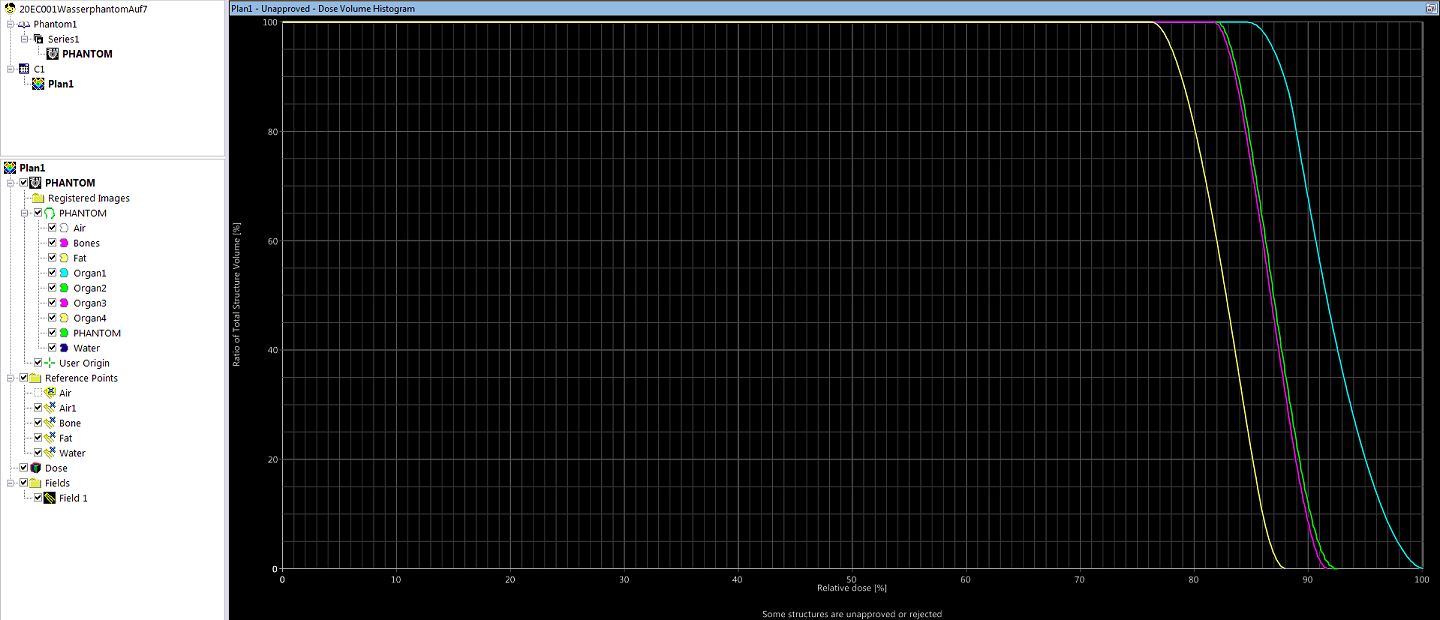
\includegraphics[width=\textwidth]{../../Wasserphantom Bilder/Aufgabe3.1_8.png}
  \caption{Dosis-Volumen-Histogramm zu den vier neu angelegten Strukturen mit dem CT-Wert Wasser.}
  \label{abb:3.1_8}
\end{figure}

Dabei liegt das Organ 1 hinter der Struktur Luft, das Organ 2 hinter Fett,
das Organ 3 hinter Wasser und das Organ 4 hinter Knochen.
Anhand des DVHs ist zu erkennen, dass in Organ 1 am meisten Dosis deponiert
wird. Etwa $100\%$ des Organs erhält eine relative Dosis von etwa $85\%$.
Die Kurven von dem Organ 2 und 3 verlaufen sehr ähnlich.
In $100\%$ dieser Organe wird mehr als $82\%$ der Dosis deponiert. In dem
letzten Organ wird am wenigsten Dosis deponiert, nämlich etwa $76\%$ der
relativen Dosis in $100\%$ des relativen Volumen.
Für die Bestrahlungsplanung folgt anhand dieser Erkenntnisse, dass
Knochengewebe im Strahlengang vermieden werden sollte, da in diesem Gewebe
viel Dosis deponiert wird und somit in dem Zielvolumen eine zu
geringe Dosis deponiert werden könnte. Außerdem ist zu erkennen, dass
Fettgewebe und Wasser als
nahezu gleich betrachtet werden können bei der Bestrahlungsplanung.
Bei Strukturen aus Luft im Strahlengang ist zu beachten, dass in diesen die
Photonenstrahlung nur wenig abgeschwächt wird und somit in den
dahinter liegenden Strukturen noch eine hohe Dosis deponiert wird. \\\\

In der Abbildung \ref{abb:3.1_9} ist zusätzlich das DVH des gesamten
Wasserphantoms in grün dargestellt.

\begin{figure}[H]
  \centering
  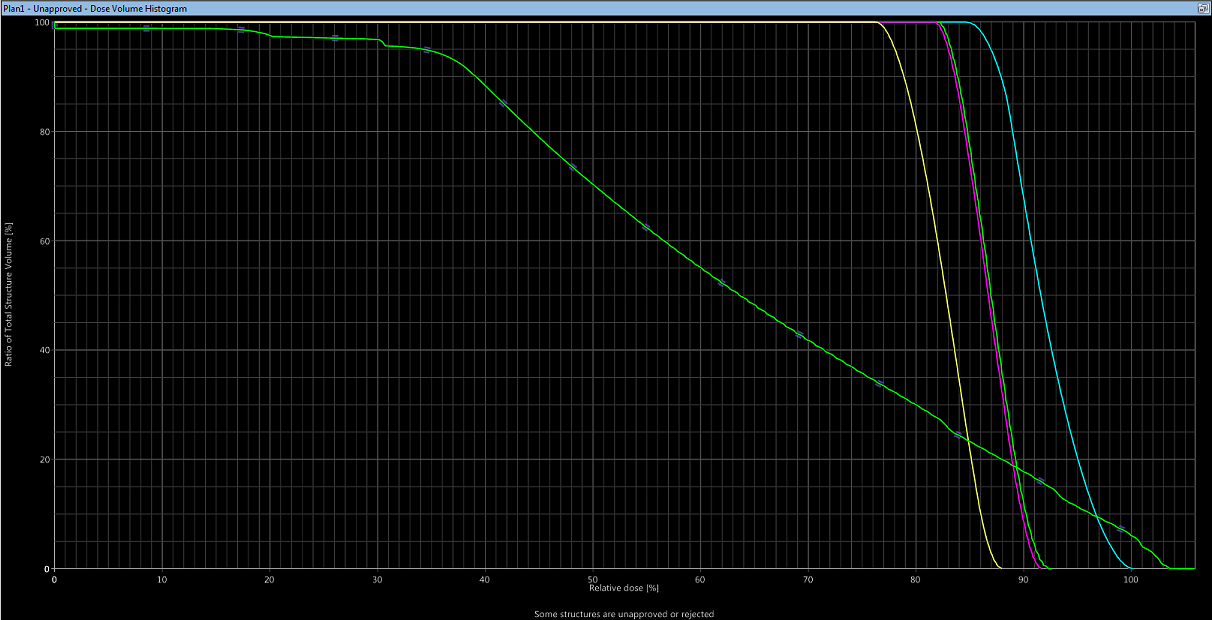
\includegraphics[width=\textwidth]{../../Wasserphantom Bilder/Aufgabe3.1_9.png}
  \caption{Dosis-Volumen-Histogramm zu den vier neu angelegten Strukturen mit dem CT-Wert Wasser und des gesamten Wasserphantoms.}
  \label{abb:3.1_9}
\end{figure}

Anhand dieser Kurve ist zu erkennen, dass etwa $70 \%$ des relativen Volumens
des Wasserphantoms eine relative Dosis von $50\%$ erhält und etwa $98\%$ eine
relative Dosis von $20\%$. Diese hohe Dosisdeposition kann mit Hilfe
des MLCs verringert werden. Die Lamellen werden dabei so eingestellt, dass
der Photonenstrahl nur im Bereich der Strukturen auf das Wasserphantom trifft.
Das neue DVH ist in Abbildung \ref{abb:3.1_10} dargestellt.

\begin{figure}[H]
  \centering
  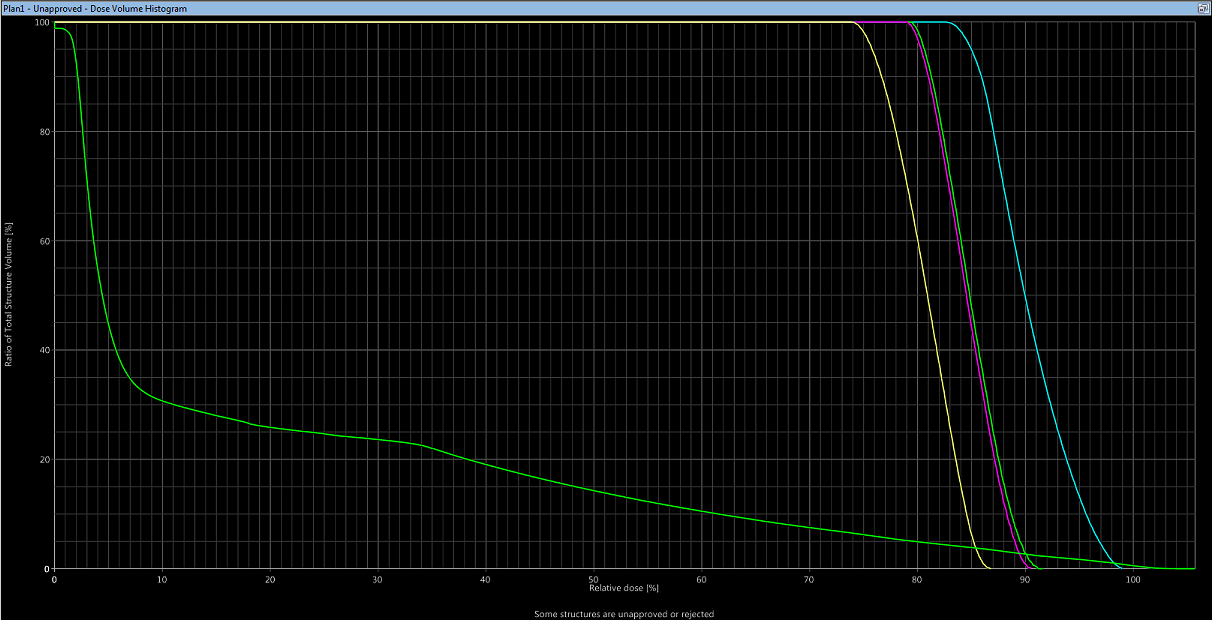
\includegraphics[width=\textwidth]{../../Wasserphantom Bilder/Aufgabe3.1_10.png}
  \caption{Dosis-Volumen-Histogramm zu den vier neu angelegten Strukturen mit dem CT-Wert Wasser und des gesamten Wasserphantoms mit MLC-begrenztem Feld.}
  \label{abb:3.1_10}
\end{figure}

Anhand dieses DVHs ist zu sehen, dass sich die Dosisdeposition in den
Organen leicht verringert. Allerdings wird dadurch in nur etwa $14\%$ des
relativen Volumens des Wasserphantoms eine relative Dosis von $50\%$ deponiert
und in $26\%$ eine relative Dosis von $20\%$.

\subsection{Tiefendosiskurven durch verschiedene Volumina}

Für diesen Teil wird erneut ein neues Wasserphantom angelegt mit den Maßen
$10$x$10$x$10$ $\si{\centi\meter\tothe{3}}$, dem Schichtabstand
$\SI{0.25}{\centi\meter}$ und einem CT-Wert von Wasser. In diesem
Wasserphantom wird im Zentrum eine Kugelförmige Struktur mit einem
Durchmesser von $d = \SI{5}{\centi\meter}$. Der CT-Wert dieser
Struktur soll den von Luft, Fett, Wasser und Knochen annehmen.
Dieses Wasserphantom wird mit einem $6$x$6$ $\si{\centi\meter\squared}$
$\SI{6}{\mega\volt}$ Photonenfeld bestrahlt bei einer Gantry Rotation von
$270°$. Nun wird eine Tiefendosiskurve entlang des Zentralstrahls
für die verschiedenen CT-Werte der Struktur aufgenommen. Da die simulierten
Werte der Tiefendosiskurven nicht aus dem Programm gespeichert werden können,
werden die hochgeladenen Werte verwendet. Diese Daten werden mittels Python
graphisch dargestellt. Die gegebenen Dosiswerte werden dabei auf das jeweilige Maximum normiert und gegen die
Tiefe x im Wasserphantom dargestellt.

\begin{figure}[H]
  \centering
  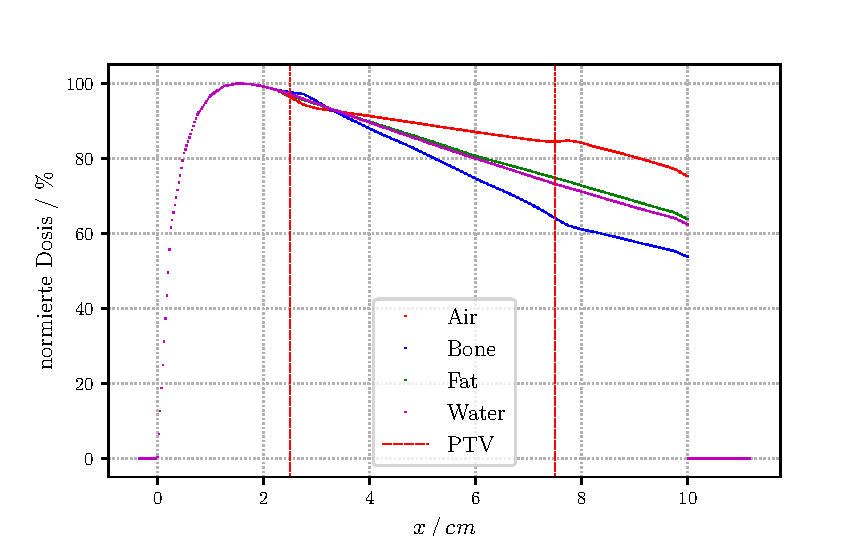
\includegraphics[width=\textwidth]{build/Aufgabe3.2.pdf}
  \caption{Normierte Tiefendosiskurven für verschiedene CT-Werte des PTVs.}
  \label{abb:3.2}
\end{figure}

Im Bereich bis zu der Struktur im Zentrum des Wasserphantoms ($0 \leq x \leq 2,5$) verlaufen
die Tiefendosiskurven alle gleich.
In dem Bereich mit den unterschiedlichen CT-Werten ($2,5 \leq x \leq 7,5$)
laufen die TDKs dann auseinander. Dabei fällt die TDK bei Knochen am stärksten, da in Knochen
die meiste Dosis deponiert wird. Jedoch steigt die Dosis bei Knochen zunächst etwas an, was an dem Dosisaufbaueffekt liegt.
Der Verlauf der TDK bei Fett und Wasser ist auch hier wieder ähnlich. Bei beiden fällt die relative Dosis linear
ab, wobei die Dosis in Wasser etwas stärker abfällt als in Fett. Deshalb laufen die TDKs bei den beiden Materialien etwas auseinander.
Das kommt daher, dass Wasser ($HU = 0$) die Photonenstrahlung etwas stärker abschwächt als Fett ($HU = -100$).
Bei Luft wird die Photonenstrahlung am wenigsten geschwächt, was an dem flachen Verlauf
der TDK zu erkennen ist. Nach der Struktur ($7,5 \leq x \leq 10$) kommt es bei Luft erneut zu
einem Dosisaufbaueffekt. Bei Fett und Wasser verläuft die TDK nahezu linear weiter,
da der Unterschied zum restlichen Wasserphantom so gering ist. Bei dem Übergang von Knochen zum
Wasserphantom ist zu erkennen, dass die TDK nach durchlaufen der Struktur nicht mehr so stark abfällt.
Generell ist in diesem Bereich zu sehen, dass die TDKs wieder den gleichen Verlauf haben, aber durch den Einfluss
der verschiedenen Strukturen nun versetzt zueinander sind.
In den Abbildungen \ref{TDK1}, \ref{TDK2}, \ref{TDK3} und \ref{TDK4} sind die einzelnen Tiefendosiskurven,
die mit dem Bestrahlungsplanungsprogramm erzeugt worden sind, noch einmal dargestellt.


\begin{figure}[H]
  \centering
  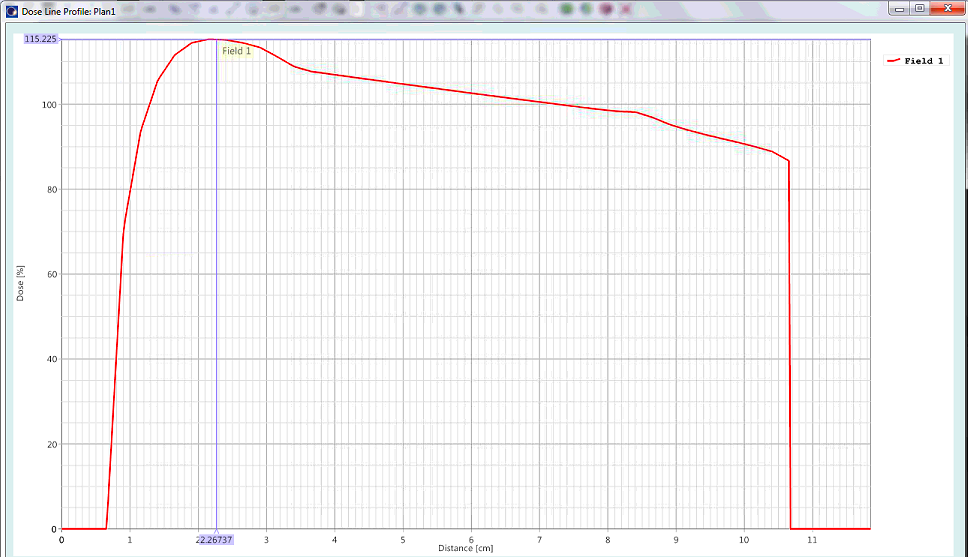
\includegraphics[width=\textwidth]{../../Wasserphantom Bilder/TDK_Luft.png}
  \caption{Tiefendosiskurve innerhalb des Wasserphantoms. In diesem Fall besteht das PTV in dem Zentrum aus Luft.}
  \label{TDK1}
\end{figure}

\begin{figure}[H]
  \centering
  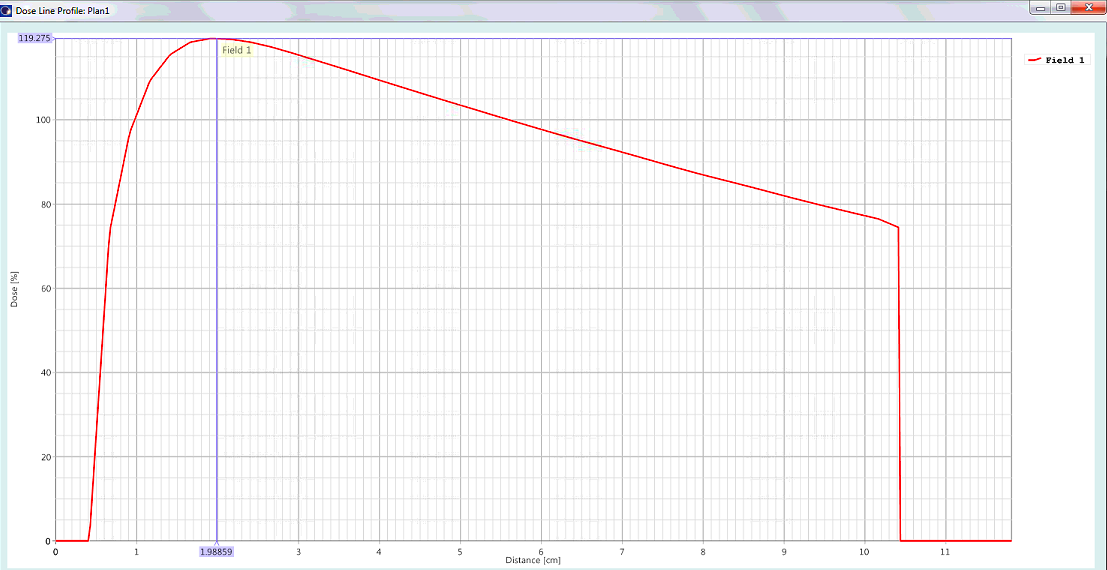
\includegraphics[width=\textwidth]{../../Wasserphantom Bilder/TDK_Wasser.png}
  \caption{Tiefendosiskurve innerhalb des Wasserphantoms. In diesem Fall besteht das PTV in dem Zentrum aus Wasser.}
  \label{TDK2}
\end{figure}

\begin{figure}[H]
  \centering
  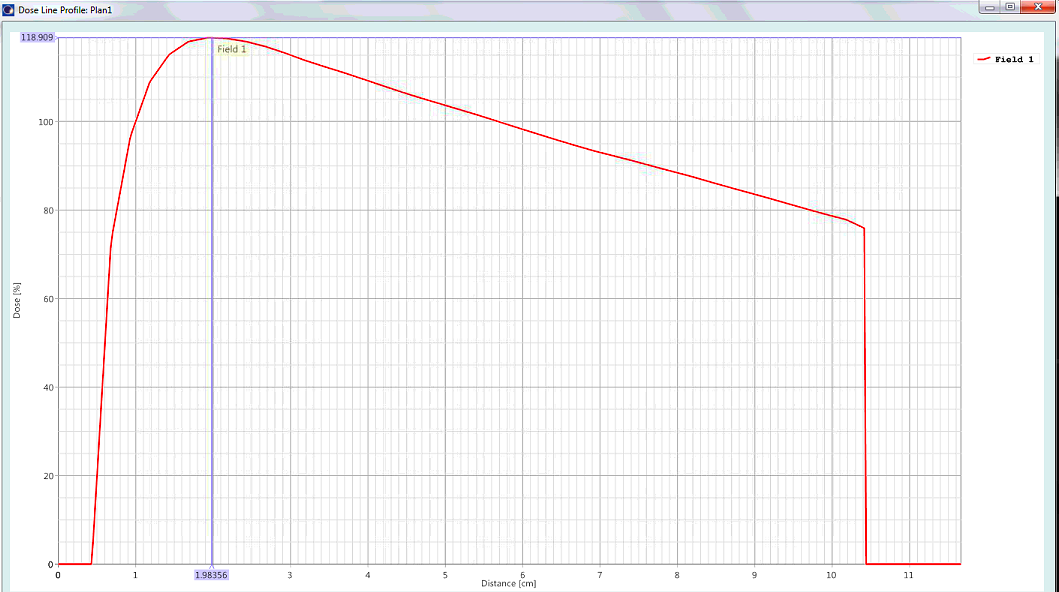
\includegraphics[width=\textwidth]{../../Wasserphantom Bilder/TDK_Fett.png}
  \caption{Tiefendosiskurve innerhalb des Wasserphantoms. In diesem Fall besteht das PTV in dem Zentrum aus Fett.}
  \label{TDK3}
\end{figure}

\begin{figure}[H]
  \centering
  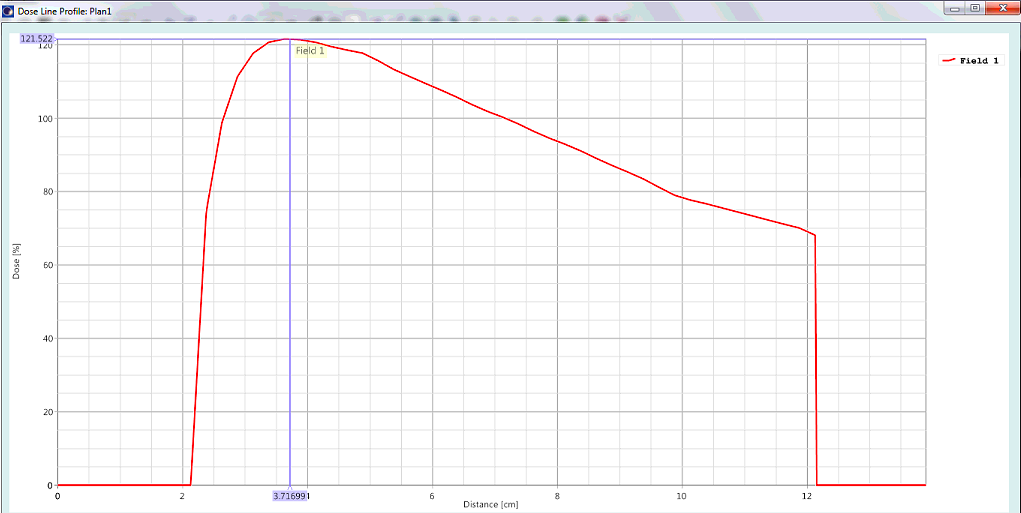
\includegraphics[width=\textwidth]{../../Wasserphantom Bilder/TDK_Knochen.png}
  \caption{Tiefendosiskurve innerhalb des Wasserphantoms. In diesem Fall besteht das PTV in dem Zentrum aus Knochen.}
  \label{TDK4}
\end{figure}
